\documentclass[project-plan]{report-template}

\usepackage{graphicx}
\usepackage{amsmath}
\usepackage{tikz}
\usetikzlibrary{arrows.meta, positioning, shapes.geometric}

\graphicspath{{./figures/}}

\university{Imperial College London}
\department{Department of Earth Science and Engineering}
\course{MSc in Applied Computational Science and Engineering}
\title{Current Content Discovery for Module Teaching}
\author{Guanyuming He}
\email{guanyuming.he24@imperial.ac.uk}
\githubusername{esemsc-gh124}
\supervisors{Sean O'Grady\\
             Rhodri Nelson}
\repository{https://github.com/ese-ada-lovelace-2024/irp-gh124}

\newcommand\casemethod{case method}

\begin{document}

\maketitlepage  

\section*{Abstract}
TBD.
\textbf{Keywords:} content discovery, information retrieval, LLM, search engines, \casemethod, Business school,

\section{Introduction}
\subsection{Problem background}
Since the emergence of Business schools in the late 19th century
\cite{first.bis.school.1, first.bis.school.2}, several distinct pedagogical
teaching strategies have been used.  First institutionalized at Harvard
Business School \cite{case.method.origin.1, case.method.origin.2}, a method
about teaching students with real world business cases (will be called
\emph{\casemethod} in the rest of the document) has been found more effective
and engaging \cite{case.method.support.1, case.method.support.2,
case.method.support.3} than traditional big lecture methods, and gained wide
adoption across the world \cite{case.method.adoption.1,
case.method.adoption.2}.

However, the case method is constrained by the availability and
collection of timely and relevant case material \cite{case.method.limit.1,
case.method.limit.3}. In particular, Christensen has identified in his classical
article that instructors would have to conduct ``extensive preparation''
\cite{case.method.limit.2} for case method, and some others emphasise the
importance of up-to-date material \cite{case.method.limit.4,case.method.limit.5}.

\subsection{Past advancements in information retrieval}
In the early 19th century, the transmission of information was still
traditional --- carried by person on paper or simply remembered. The invention
of telegraph in the 1840s by Morse, Cornell, and Henry
\cite{history.telegraph.1, history.telegraph.2}, was perhaps the first big
advancement in history. This technological innovation was considerably improved
by the invention of the telephone by Bell in 1876 \cite{history.telephone.1,
history.telephone.2}.

Wired communication is critically limited by geographical
features on where the wires were laid. Around the late 19th century, 
Marconi's experiments with wireless telegraphy \cite{history.wireless.1}
introduced electromagnetic wave-based wireless communication, eventually
accumulating into the world's first voice broadcast by radio in 1906
\cite{first.voice.broadcast}. 

The next many decades have seen people improving on the serious limitations of
the communication methods. \cite{wireless.weakness.1, wireless.weakness.2,
wireless.weakness.3}.  Theoretically, Hartley observed a logritham pattern of
information capacity \cite{hartley.log.information} and then Shannon expanded
on it to first define \emph{bits} and \emph{entropy}, giving a formal
mathematical theory of information \cite{shannon.theory.communication} in 1948.
Another notable discovery was modulation techniques \cite{history.modulation}. 

As the theoretical understanding of information progressed, people began to
have the idea of \emph{searching} for information based on content
and by relevance, instead of by unique identifier
\cite{history.information.retrieval}. The term \emph{information
retrieval} was coined by Mooers in 1950
\cite{mooers.info.ret.term}. Since then, information retrieval systems have
quickly evolved, and Griffiths and King identified four phases of its
evolvement: ``(1) manual and mechanical
devices; (2) offline computing; (3) online computing, vendor access; (4)
distributed, networked, and mass computing.'' \cite{info.ret.4.phases}, with
the last three substantially contributed to by the invention of the Internet
\cite{history.internet}, and consequently the emergence of search engines in
the 1990s \cite{history.search.engines, history.internet.search.engines}.
Henceforth, search engines greatly expanded in speed and
coverage and has been significantly impacting the society's information for at
least a decade \cite{search.engine.impact.1, search.engine.impact.2}.

Recently, LLMs have had a huge impact on various areas \cite{llm.impact.1}. One
strong appeal of LLMs is that they could easily work with natural language
input \& output \cite{llm.power.1, llm.power.2}. However, some argue that they
could not inherently
reason about what they output \cite{llm.limit.1, llm.limit.2, llm.limit.3}.
Indeed, hallucination \cite{llm.hallucination.1, llm.hallucination.2} and other
forms of distortion of facts, is a big problem of LLMs. On the other hand,
although search engines rely on determinstic algorithms that give precise
reference to searched result, they could not compare with LLMs' NLP abilities.

Therefore, it is a current research direction to integrate LLMs with search
engines \cite{llm.meet.search.1, llm.meet.search.2, llm.meet.search.3}.
Specifically, Xiong et al.\ proposes to categorize them into ``LLM4Search'' and
``Search4LLM'', where ``A4B`` means using A to improve B
\cite{llm.meet.search.1}. Here is where my thesis will build upon.  

\subsection{Goals}
In this project, I will attempt to improve the current state of information
retrieval further by designing and developing a software system. More
precisely, these are the goals:
\begin{enumerate}
	\item By combining LLMs and search engines, compensate each other's
		weakeness in information retrieval.
		\begin{enumerate}
		\item The system shall be able to take unstructured data describing the
		desired kinds of information.
		\item The system shall improve LLMs on result credibility and
			interpretibility. 
		\end{enumerate}
	\item Enhance the automation of the current general public information
		retrieval tools so that	user would only need to occasionally configure
		the system to run them.
	\item Specially tailor the system to business teaching related information,
		aiming to gather information from authentic and reliable sources.
	\item The system shall support up-to-date information retrieval. More
		precisely, the system shall support a specification of desired time
		range.	
	\item The system could support user feedback and learning from it to
		provide information more close to one's need.
\end{enumerate}

\section{Methods} 
\subsection{Architecture}
Based on the goals, the system is designed to be a chain of tools invoking each
other.

What directs the system is the user's configuration, which is expected to
include
\begin{enumerate}
	\item A time range of information to retrieve.
	\item A description of the types of information to
		retrieve.
	\item How the retrieved information is sent to the user.
	\item A frequency of running the tool.
\end{enumerate}

Based on the configured running frequency, the tool will
\begin{enumerate}
	\item Use LLMs to translate the configured description and generate a list
		of search engine prompts.
	\item The prompts are fed to search engines, with the configured time
		constraint.
	\item The search results are gathered and processed. How the information is
		processed and filtered may rely on other AI systems like a
		rule-based expert system.
	\item The processed results may be summarized by LLMs.
	\item The results are sent to the users via the configured ways.
	\item Optionally, the user gives feedback to the results. The tool can
		thus improve on feedback
\end{enumerate}

Figure~\ref{fig.arch.flow} demonstrates my architecture design and the workflow
of the system.

\begin{figure}[htbp]
\centering
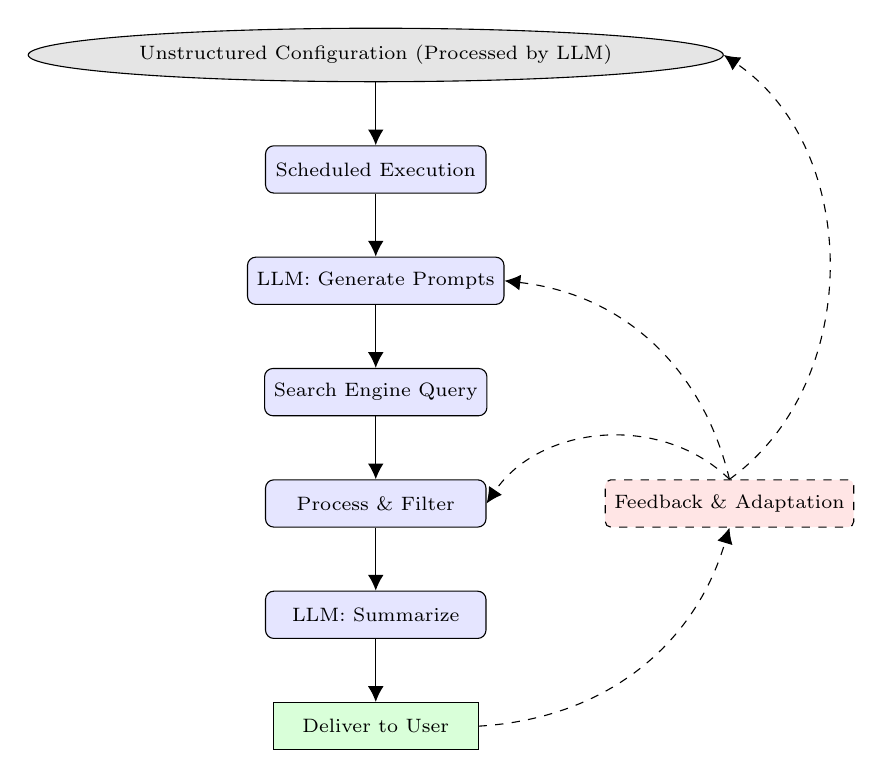
\begin{tikzpicture}[
	  node distance=0.8cm,
  every node/.style={font=\scriptsize},
  process/.style={draw, rounded corners=3pt, fill=blue!10, minimum width=2.8cm, minimum height=0.6cm, text centered},
  input/.style={draw, ellipse, fill=gray!20, minimum width=2.6cm, minimum height=0.6cm},
  output/.style={draw, rectangle, fill=green!15, minimum width=2.6cm, minimum height=0.6cm},
  feedback/.style={draw, dashed, fill=red!10, rounded corners=2pt, minimum width=2.6cm, minimum height=0.6cm},
  arrow/.style={-{Latex[width=2mm,length=2mm]}, line width=0.5pt},
  fb/.style={-{Latex[width=2mm,length=2mm]}, line width=0.4pt, dashed, bend right=35}
]

% Main vertical flow
\node[input] (config) {Unstructured Configuration (Processed by LLM)};
\node[process, below=of config] (scheduler) {Scheduled Execution};
\node[process, below=of scheduler] (promptgen) {LLM: Generate Prompts};
\node[process, below=of promptgen] (search) {Search Engine Query};
\node[process, below=of search] (processresults) {Process \& Filter};
\node[process, below=of processresults] (summarize) {LLM: Summarize};
\node[output, below=of summarize] (deliver) {Deliver to User};
\node[feedback, right=1.5cm of processresults] (feedback) {Feedback \& Adaptation};

% Arrows (main flow)
\draw[arrow] (config) -- (scheduler);
\draw[arrow] (scheduler) -- (promptgen);
\draw[arrow] (promptgen) -- (search);
\draw[arrow] (search) -- (processresults);
\draw[arrow] (processresults) -- (summarize);
\draw[arrow] (summarize) -- (deliver);

% Feedback arrows (clean curves)
\draw[fb] (deliver.east) to (feedback.south);
\draw[fb] (feedback.north) to (promptgen.east);
\draw[fb] (feedback.north) to [bend right=50] (processresults.east);
\draw[fb] (feedback.north) to [bend right=55] (config.east);
\end{tikzpicture}
\caption{Architecture and operational flow of the software system}
\label{fig.arch.flow}
\end{figure} 	

\subsection{Implementation plan}
In this section, I give the plan of my implementation. It is only meaningful
for the project plan, as it will be replaced by the specifics in the final
report.

\subsubsection{Configuration format} 
LLMs have demonstrated unprecedented ability to process unstructured data
\cite{llm.unstructured.data.1, llm.unstructured.data.2}. Thus, it is desirable
for the system to accept unstructured configuration from the user. The user may
give a natural language description of the wanted information, some
examples, e.g., URLs, or simply the teaching slides and videos
from previous classes.

Nevertheless, there are a few configurations that must be formatted.
\begin{enumerate}
	\item A range of time for the information retrieved.
	\item (Optional) A list of sources (e.g. websites) to always include or exclude.
	\item The destination of the collected information (e.g. email addresses of
		teaching staff).
\end{enumerate}
Of course, LLMs can still try to infer them from the given unstructured data,
but they must be presented to the user for her to decide and correct, because
these configurations are strict and a little error will have great effects.

Another important output from unstructured configuration is the search prompts
or insturctions generated by the LLMs. As this output direct controls the
information retrieved. LLMs for this task will be specifically tuned to ensure
\begin{itemize}
	\item Diversity of results.
	\item A specific distribution of results. E.g., a more authentic website
		will contribute relatively more information.
\end{itemize}

\subsubsection{Searching implementation} 
One problem of search engine APIs is that they have ungenerous search limits
\cite{search.api.limit.1}, allowing about 1000 queries per month, which is not
enough for frequent testing and prototyping.

As a result, I plan to use some other self-developed system in parallel with
search engines, which do only a small amount of tasks that truly require whole
Internet searching. The majority of the searching will be handled by scraping a
limited sets of websites, most likely.

\subsubsection{Content processing \& filtering} The content processing could
utilize content deduplication, relevance scoring, and source credibility
assessment.  The processing pipeline will need to handle various content
formats including urls, texts, images, and videos.

\subsubsection{Summarization tuning} Processed results will be summarized
with business-focused prompting strategies. It is where the system
will be seriously tuned to avoid hallucination and ensure the completeness of
the summary.

\subsubsection{Information delivery} Results shall be sent to users via
configured methods, which may include email addresses or
educational/collaboration online platforms. The delivery component shall handle
different user preferences and ensure information is presented in a format
suitable for educational use.

\subsubsection{Feedback system} The system shall collect user
feedback to improve
future searches. This involves designing feedback mechanisms that capture both
explicit user ratings and implicit behavioral signals. Possible algorithms
include recommendation algorithms and other machine learning models.

\subsection{Technical considerations} 
The system will be a high-level program, which benefits from simple programming
languages like Python. On the other hand, the system may have specific
performance requirements, especially for LLMs and other machine learning
algorithms. The likely result is then a combination of different programming
languages and technical frameworks.

\subsection{Evaluation and validation} 
It may be desirable to develop an external evaluation framework for the system,
if I have enough time in the end. My supervisor my also have people to provide
external human feedback.

\clearpage

% References
\bibliographystyle{plain}
\bibliography{references.bib}  % BibTeX references are saved in references.bib

\end{document}          
